
%% ============================================================
%%  CHƯƠNG 3: PHƯƠNG PHÁP THỰC HIỆN
%% ============================================================
\chapter{Phương pháp thực hiện}

Các phương pháp FD hiện tại hỗ trợ hiệu quả các kiến trúc mô hình không đồng nhất, nhưng chúng hoặc vẫn dễ bị thao túng Byzantine, phụ thuộc vào điều phối tập trung, hoặc sử dụng một mô hình thứ hai để hỗ trợ tiết chế các dự đoán nhãn công khai kém tự tin. Để giải quyết các thách thức này, DFD-IDS là phương pháp đề xuất, bao gồm chắt lọc kiến thức liên kết phân tán kết hợp cơ chế tiết chế dựa trên năng lượng, Chắt lọc kiến thức dựa trên bằng chứng, tổng hợp logits chống tấn công Byzantine và lựa chọn phần tử điều phối phân tán. Trong DFD-IDS, các client tinh chỉnh mô hình qua học giám sát cục bộ và trao đổi các dự đoán được tiết chế bằng năng lượng trên một tập dữ liệu công khai. Một phần tử điều phối, được bầu chọn mới ở mỗi vòng liên kết từ các client, thu thập các dự đoán này cùng với một mặt nạ nhị phân biểu diễn giá trị tiết chế. Sau đó, logit của các client được lọc bằng thuật toán tổng hợp Blom Robust Filter được đề xuất. Cuối cùng, kiến thức tổng hợp được phân phối lại cho các client để thực hiện Chắt lọc kiến thức dựa trên bằng chứng trước khi chuyển sang vòng học tiếp theo.

\begin{figure*}[ht]
    \centering
    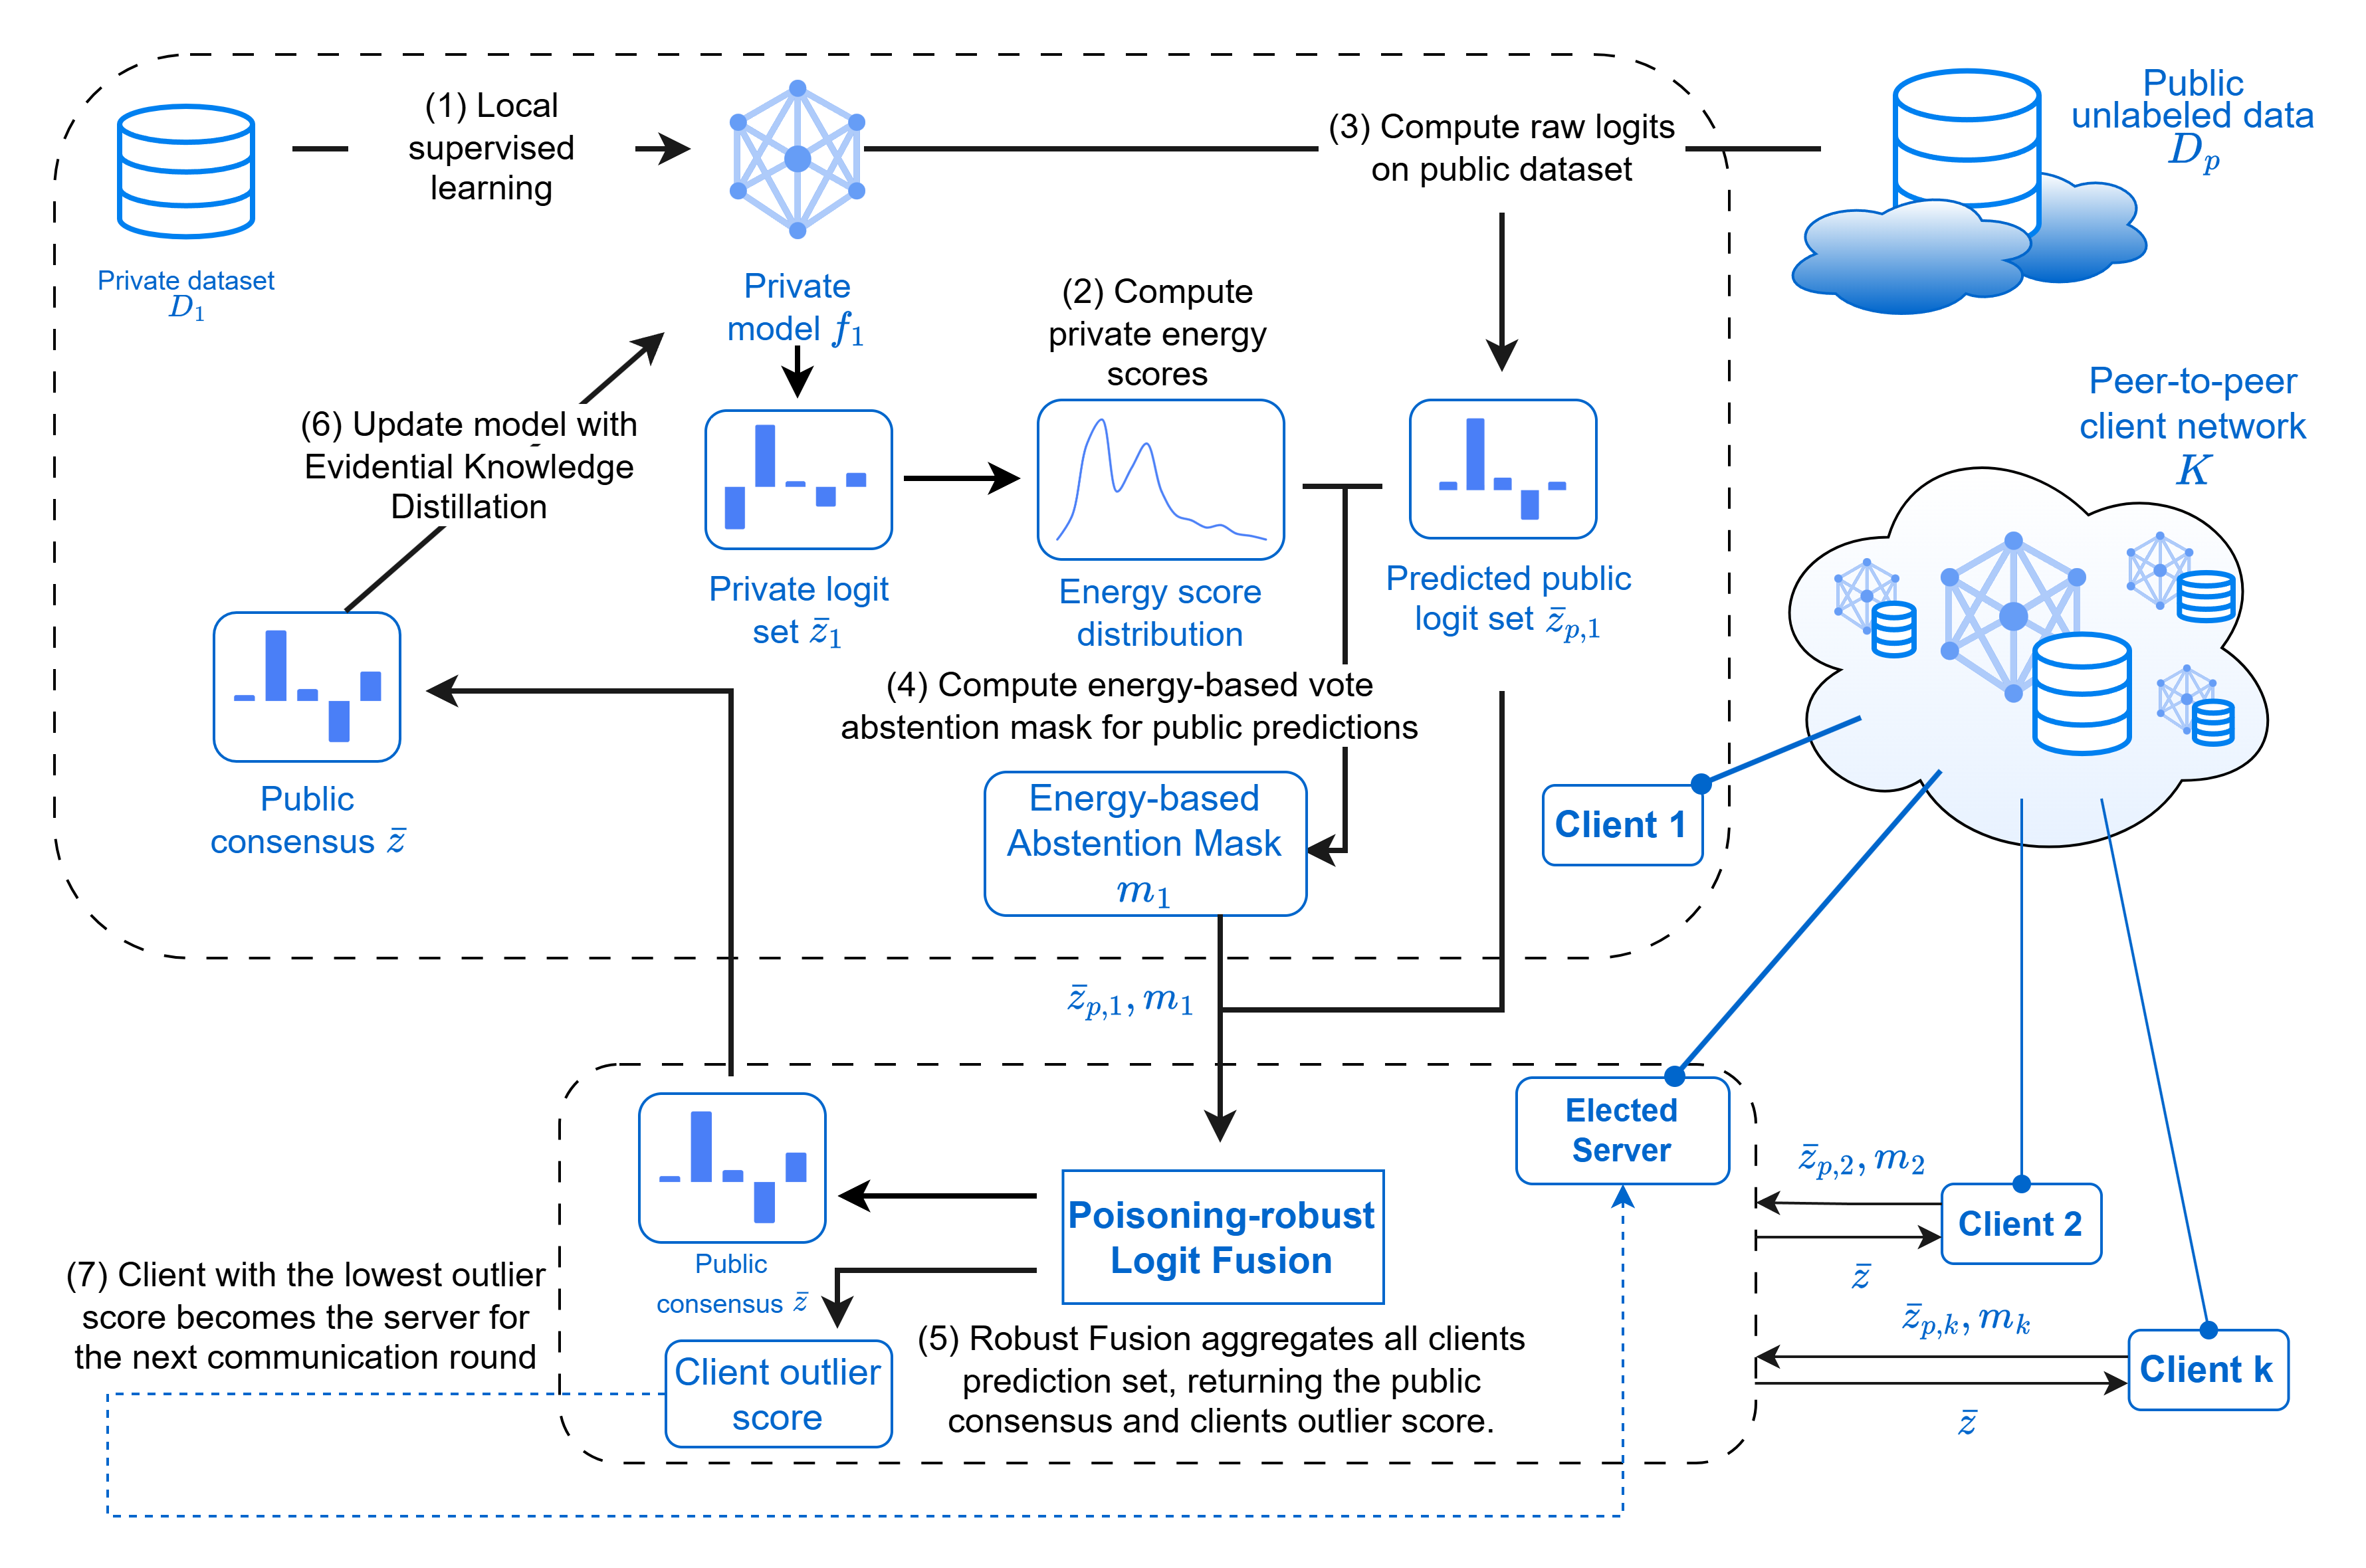
\includegraphics[width=0.9\textwidth]{images/Pipeline.png}
    \caption{Workflow của khung giải pháp DFD-IDS.}
    \label{fig:pipeline}
\end{figure*}

\section{Tổng quan hệ thống}
\label{sec:system_overview}

Vào đầu mỗi vòng học liên kết, mỗi client $k$ thực hiện huấn luyện có giám sát cục bộ trên tập dữ liệu riêng của mình, tạo ra bộ logit $\bar z_k$ là dự đoán của mô hình trên tập dữ liệu cục bộ. Mô hình kết quả sau đó được sử dụng để đánh giá các mẫu từ tập dữ liệu công khai chia sẻ, tạo ra bộ logit $\bar z_{p,k}$là dự đoán của mô hình trên tập dữ liệu công khai.

Từ bộ logit $\bar z_k$, mô hình sử dụng thuật toán \ref{energy} để sinh ra phân phối energy và chọn lọc dự đoán có độ tự tin cao trong $\bar z_{p,k}$. Quá trình này được mô tả chi tiết trong phần \ref{sec:eva}.

Phần tử điều phối thực hiện tổng hợp các bộ logit sử dụng Robust Logit Fusion như phần \ref{sec:blom} đề xuất để xác định các dự đoán độc hại và tổng hợp bộ dự đoán đã được lọc các cập nhật độc hại. Phần tử điều phối tính điểm cho mỗi client từ kết quả lọc bằng một mặt nạ nhị phân $o_k$, tăng dần khi dự đoán của nó bị lọc. Chỉ những client có điểm thấp hơn ngưỡng đặt ra mới được giữ lại, và các dự đoán của chúng cũng phải vượt qua bước lọc trước đó để tham gia kết hợp logits cuối cùng. Các điểm số này cũng được sử dụng để xác định bộ điều phối trong vòng truyền thông tiếp theo.

Các logits tổng hợp được phân phối lại cho tất cả các client tham gia cho giai đoạn Chắt lọc kiến thức dựa trên bằng chứng, trước khi tiến hành vòng truyền thông tiếp theo.

\section{Cơ chế Energy-based Vote Abstention (EVA)}
\label{sec:eva}

Các khung giải pháp chắt lọc kiến thức liên kết hiện tại như FedMD \cite{li2019fedmd} và FedDistill \cite{roux2025byzantine} thường xử lý tất cả các mẫu công khai như nhau trong quá trình trao đổi kiến thức. Trong môi trường Non-IID khắc nghiệt như dữ liệu mạng, tập dữ liệu công khai thường chứa các mẫu của các lớp thiểu số nằm ngoài phân phối của đa số clients. Do đó, các client này tạo ra các dự đoán thiếu sự chắc chắn trên những mẫu thuộc các lớp mà chúng chưa từng thấy, ảnh hưởng tiêu cực tới chất lượng của bộ logit được tổng hợp. Việc chắt lọc kiến thức từ một bộ logit chất lượng suy giảm như vậy ảnh hưởng rất nặng lên mô hình học.

Để xử lý vấn đề này, phương pháp đề xuất cơ chế EVA. Mỗi client tính toán điểm năng lượng trên tập dữ liệu riêng của mình sử dụng Eq. \ref{energy}, được coi là phân phối nội tại (in-distribution). Sau đó, phân vị (quantile) thứ $q$ của điểm năng lượng cục bộ được chọn làm ngưỡng tin cậy riêng cho từng client:

\begin{equation}
\label{eva}
\tau_k=Q_q(\{E(x) | x \in D_k\})
\end{equation}

trong đó $Q_q$ là phân vị thứ $q$. Nghiên cứu phát hiện OOD dựa trên năng lượng \cite{liu2020energy} đánh giá hiệu suất sử dụng chỉ số FPR95, đo tỷ lệ False Positive khi True Positive của các mẫu in-distribution được cố định ở 95\%. Dựa vào đó, phương pháp đề xuất cũng cấu hình phân vị của EVA là thứ $95$. Ngưỡng phân vị này phải cân đối giữa các giá trị energy cao đến từ các mẫu khó học trong phân phối dữ liệu cục bộ, cũng không được quá thấp để tránh tiết chế các dự đoán hoàn toàn có đủ độ tự tin của mô hình cục bộ.

Vì cơ chế EVA phụ thuộc hoàn toàn vào mô hình cục bộ và dữ liệu cục bộ, cơ chế này thích ứng tự nhiên với ngữ cảnh đa kiến trúc mô hình và bất đồng phân phối dữ liệu.

Tuy nhiên, trong các kịch bản Byzantine, các tác nhân Byzantine xem như bỏ qua cơ chế EVA này để tối đa hóa bề mặt tấn công. Nếu cơ chế EVA tiết chế hoàn toàn các dự đoán cục bộ từ phía client, các mẫu công khai thuộc nhãn hiếm sẽ bị các dự đoán của tác nhân Byzantine chiếm đa số, dẫn đến việc bộ lọc mất hiệu quả. Để giải quyết hạn chế này, mỗi client khởi tạo một mặt nạ nhị phân làm trọng sổ tổng hợp để đi kèm với toàn bộ dự đoán:

\begin{equation}
\label{energymask}
m_k(x) =
\begin{cases}
1,  &E_k(x) \leq \tau_k \\
0, &\text{otherwise}
\end{cases}
\end{equation}

\section{Robust Logit Fusion}
\label{sec:blom}

\subsection{Quy trình hoạt động}
Sau khi các bộ logit dự đoán trên tập dữ liệu công khai được thu thập từ tất cả clients, phần tử điều phối tiến hành tổng hợp logit. Khi một phần clients là Byzantine gửi các dự đoán được tạo ra một cách đối nghịch, việc tổng hợp đơn giản (ví dụ: tổng hợp trung bình) sẽ trả về một bộ logit bị đầu độc. Thay vì đó, một quy trình tổng hợp hai lớp được đề xuất như trong Thuật toán \ref{alg:RobustFusion}. Các dự đoán của client trước tiên được lọc bằng Bộ lọc Blom Robust Filter cho mỗi mẫu công khai $x \in D_P$. Nếu bộ lọc từ chối dự đoán của client $k$ cho mẫu $x$, một mặt nạ nhị phân theo từng mẫu $o_k(x)$ riêng cho mỗi client được đặt thành 1. Sau khi tất cả các mẫu công khai được xử lý, các client có điểm ngoại lai $\frac{1}{|D_p|}\sum_{x \in D_p}o_k(x)$ cao hơn tham số đặt trước $\varepsilon$ sẽ bị loại bỏ và lượt đầu tiên hoàn thành. Các client còn lại bước vào lớp tổng hợp thứ hai, tổng hợp các dự đoán của tập client này thành một bộ logit sau cùng $\bar z(x)$, được tính như sau:

\begin{equation}
\label{FinalFusion}
\bar z(x)=\frac{1}{|K|}\sum_{k \in K}m_k(x) (1-o_k(x))\cdot z_k(x)
\end{equation}

trong đó $m_k(x)$ là mặt nạ bỏ phiếu trắng của client $k$ cho mẫu công khai $x$ được tính bằng EVA, $o_k(x)$ là mặt nạ ngoại lai nhị phân, và $z_k(x)$ là vector logit của $k$ trên mẫu $x$.

\begin{algorithm}[H]
\label{alg:RobustFusion}
\caption{Robust Logit Fusion}
\KwIn{Dự đoán của clients trên các mẫu công khai $S(x),x \in D_p,S(x)=\{z_1,\ldots,z_{|K|}(x)\}$, mặt nạ EVA $m_k(x), \forall x \in D_p, \forall k \in K$, ngưỡng $\varepsilon$}
\KwOut{Consensus $\bar z = \{ \bar z(x) | x \in D_p\}$}

Khởi tạo $o_k = \{o_k(x)|o \in [0,1]\,x \in D_p\}$, $o_k(x)=0, \forall k \in K$\;

\ForEach{mẫu công khai $x$}{
    Lọc client Byzantine bằng \texttt{BlomRobustFilter} (Thuật toán \ref{alg:BlomRobustFilter})\;
    $K^a \leftarrow \text{BlomRobustFilter}(S(x),K)$\;
    \ForEach{client $k \in K$}{
        \If{$k \notin K^a$}{
            $o_k(x) = 1$\;
        }
    }
}

Cập nhật $K = \{k \in K | \frac{1}{|D_p|}\sum_{x \in D_p}o_k(x) \leq \varepsilon\}$ \;

\ForEach{mẫu công khai $x$}{
Tổng hợp consensus $\bar z(x)$ qua Eq.\ref{FinalFusion}\;
}
\Return{$\bar z$, $o_k$}
\end{algorithm}

\subsection{Blom Robust Filter}
\label{sub:blom_spectral}

Một phương pháp FD có cùng cơ chế chống tấn công Byzantine là Cronus \cite{chang2019cronus}, bằng cách ứng dụng RobustFilter \cite{diakonikolas2017robustfilter} để tổng hợp logits. RobustFilter của Cronus đã thành công trong việc chống các tấn công Byzantine nâng cao như ALIE \cite{baruch2019little}, tuy nhiên hoạt động kém hơn so với tổng hợp trung bình trong ngữ cảnh lành tính. Trong thuật toán gốc, họ chọn một ngưỡng eigenvalue cố định là 9 và ma trận dự đoán được coi là lành tính nếu eigenvalue cao nhất của nó không vượt quá ngưỡng này. Việc chọn một ngưỡng cố định cho eigenvalue lớn nhất không lý tưởng, vì độ lớn của eigenvalue lớn nhất phụ thuộc vào cấu trúc covariance, kích thước client tham gia và số chiều của không gian logit.

Thay vì đặt ngưỡng trực tiếp trên eigenvalue cao nhất phụ thuộc vào số chiều, các dự đoán của client được biến đổi thành độ lệch chuẩn hóa bất biến với phép dịch chuyển và tỷ lệ. Với eigenvector $v$ lớn nhất của ma trận dự đoán $S(x) = \{z_k(x)|k \in K\}$ trên một mẫu $x$ duy nhất, và vector dự đoán trung bình $\bar z(x)$, mỗi vector logit của client được chiếu dọc theo $v$ thành một giá trị vô hướng:

$$s_k(x) = v^\top(z_k(x) - \bar z(x))$$

và các giá trị này được chuẩn hóa thành độ lệch sử dụng median absolute deviation:

$$\mathrm{d}_k(x) = \frac{|s_k(x) - \tilde s_k(x)|}{k \cdot \text{median}_{k \in K}|s_k(x) - \tilde s(x)|}$$

trong đó $k=1/(\Phi(3/4)) \approx 1.4826$.

Sau khi chuẩn hóa, các độ lệch đã có thể so sánh được mà không phụ thuộc vào số client và số chiều của logit dự đoán. Do đó, việc đặt ngưỡng eigenvalue được thay thế bằng mô hình tham chiếu thống kê dựa trên thứ hạng. Các độ lệch của client được sắp xếp theo thứ tự tăng dần $\mathrm{d}_{(1)} \leq \ldots \leq \mathrm{d}_{(|K|)}$. Độ lệch $d_{r}$ ở mỗi thứ hạng $r$ được so sánh với giá trị kỳ vọng $b_r$ của nó dưới phân phối Half-normal cumulative distribution. Thống kê thứ tự Blom \cite{blom} được sử dụng để ước lượng giá trị kỳ vọng của từng thứ hạng trên phân phối này từ nghịch đảo xác suất:

$$b_r = \Phi^{-1}\left(\frac{1}{2} + \frac{1}{2} \cdot\frac{r-\alpha}{|K| - 2\alpha +1} \right)$$

trong đó $\alpha = 0.375$. Do thống kê Blom trên phân phối Half-normal cumulative distribution rất nhạy trước các giá trị lệch mạnh, các client Non-IID lành tính có dự đoán khác so với đa số đôi khi có thể bị loại bỏ. Sự đánh đổi này là có chủ ý, vì các kỹ thuật tấn công Byzantine gần đây đã phát triển để khai thác tính không đồng nhất tự nhiên của các tập dữ liệu liên kết nhằm che giấu các cập nhật độc hại trong biến động Non-IID tự nhiên như Hidden-in-plain-sight (HIPS) \cite{roux2025byzantine} hoặc tự điều chỉnh mức tấn công để tiệm cận gần trung tâm của bộ tổng hợp ở các vòng liên kết trước \cite{xie2025poisonedfl}.

\begin{algorithm}[H]
\label{alg:BlomRobustFilter}
\caption{Bộ lọc Blom Robust}
\setstretch{1.15}
\KwIn{Dự đoán của clients trên một mẫu $x$ $S(x) = \{z_k(x)|k\in K\}, S(x) \in \mathbb{R}^{|K| \times |C|}$, tập client đang hoạt động $K^a \subseteq K $}
\KwOut{Tập client được chấp nhận $K^a$}
\While{True}{
    Gọi $S^a(x) = \{z_k(x)|k\in K^a\}$ là tập dự đoán của client đang hoạt động\;
    Tính trung bình $\bar z^a(x)$ và hiệp phương sai $\Sigma_{S^a}$\;
    Tìm eigenvector $v$ hàng đầu của $\Sigma_{S^a}$ với eigenvalue cao nhất $\lambda_{max}(\Sigma_S)$ \\
    $v(x) = \arg\max_{||\textbf{u}||=1} \textbf{u}^\top \Sigma_S \textbf{u}$\;
    Chiếu dự đoán mỗi client $k$ dọc theo $v$ thành giá trị vô hướng \\
    $s_k^a(x)=v^\top(z_k^a(x)-\bar z^a(x))$\;
    Tìm trung vị của phép chiếu $\tilde s^a(x) = \text{median}_{k \in K^a}s_k(x) $\;
    Tìm ước lượng tỷ lệ dựa trên MAD \\
    $\sigma^a(x) = 1.4826 \cdot \text{median}_{k \in K^a}|s_k^a(x) - \tilde s^a(x)|$\;
    Tính độ lệch chuẩn hóa tuyệt đối cho mỗi client \\
    $\mathrm{d}_k^a(x) = \frac{|s_k^a(x)-\tilde s^a(x)|}{\sigma^a(x)}$\;
    Tính giá trị kỳ vọng Blom cho thống kê thứ tự $r$ của $K^a$ biến chuẩn hóa \\
    $b_r^a = \Phi^{-1} \left(\frac{1}{2} + \frac{1}{2} \cdot\frac{r-0.375}{|K^a| + 0.25} \right), r=1,\ldots,|K^a|$\;
    Sắp xếp các client đang hoạt động theo $\mathrm{d}_k^a(x)$ tăng dần; đặt $\mathrm{d}_{(1)} \leq \cdots \leq \mathrm{d}_{(K^a)}$ là dãy đã sắp xếp với tham chiếu Blom $b_1^a \leq \cdots \leq b_{|K^a|}^a$\;
    Định nghĩa khối hòa (tie block) của thứ hạng $r$ là $\mathcal{T}(r) = \left\{ r' : \mathrm{d}_{(r')} = \mathrm{d}_{(r)} \right\}$\;
    Loại bỏ client ở thứ hạng $r$ nếu $\;\exists\, r' \in \mathcal{T}(r)$ sao cho $\mathrm{d}_{(r')} > b_{r'}^a$\;
    $K^a \leftarrow K^a \setminus \bigl\{k_{(r)} : \exists\, r' \in \mathcal{T}(r),\; \mathrm{d}_{(r')} > b^a_{r'}\bigr\}$\;
    \textbf{if} $K^a$ unchanged \textbf{or} $|K^a| \leq \lfloor\frac{|K|}{2}\rfloor$ \textbf{then break};
}
\Return{$K^a$}
\end{algorithm}

\section{Lựa chọn phần tử điều phối}
\label{sec:server_selection}

Các phương pháp chắt lọc kiến thức liên kết thông thường giả định một máy chủ trung tâm đáng tin cậy chịu trách nhiệm thu thập và tổng hợp dự đoán của clients. Giả định này tạo ra một điểm nghẽn trong hệ thống thực tế. Để loại bỏ sự phụ thuộc vào một bộ điều phối duy nhất, một hệ thống liên kết phân tán theo kiến trúc star được áp dụng, trong đó việc chỉ định làm phần tử điều phối liên tục thay đổi giữa các clients tham gia.

Trong vòng học liên kết đầu tiên, tất cả clients ngẫu nhiên chọn ra một phần tử điều phối. Client được chọn đóng vai trò là phần tử tổng hợp tạm thời, cùng với các ứng viên bổ sung đóng vai trò là bộ điều phối dự phòng trong trường hợp client được chọn dropout.

Trong các vòng tiếp theo, việc lựa chọn bộ điều phối được quyết định bởi kết quả của bộ lọc Blom Robust Filter (\ref{alg:BlomRobustFilter}). Client có tần suất bị lọc thấp nhất được bầu làm máy chủ tổng hợp cho vòng tiếp theo, trong khi các client có tần suất bị lọc gần với điểm thấp nhất được bầu làm dự phòng.

\section{Evidential Knowledge Distillation trong DFD-IDS}
\label{sec:ekd_dfdids}

Sau khi quá trình kết hợp logits hoàn tất trong DFD-IDS, mỗi client, với consensus $\bar{z} = \{\bar{z}(x)|x \in D_p\}$ đã nhận và tập logits dự đoán riêng $\bar z_{p,k} = \{z_k(x), x \in D_p\}$, chắt lọc kiến thức từ consensus bằng phương pháp chắt lọc kiến thức EKD. Chúng tính toán vector tham số Dirichlet cho mỗi vector consensus và vector logits tương ứng:

$$\alpha^T = \exp(\bar z(x)) + \lambda_{\text{weight}}$$
$$\alpha^S = \exp(z_k(x)) + \lambda_{\text{weight}}$$

trong đó $\exp()$ là hàm mũ, $\lambda_{\text{weight}}$ là trọng số tiên nghiệm và $\lambda_{\text{weight}}=1$ được chọn. Sau đó, mỗi client chắt lọc kiến thức bằng cách tối ưu hóa hàm mất mát (\ref{ekd}) cho tất cả các mẫu công khai $x$ với consensus và vector dự đoán tương ứng.

\begin{algorithm}[H]
\label{alg:dfd_ids}
\caption{DFD-IDS}
\KwIn{Tập client phân tán $K$, tập dữ liệu riêng $D_k, \forall k \in K$, tập dữ liệu công khai không nhãn $D_p$, mô hình client $f_k$ với tham số $w_k$, ngưỡng $\varepsilon$, số vòng liên kết $t \in T$}
Khởi tạo máy chủ tổng hợp tạm thời và dự phòng, $k_s, k_b \leftarrow RNG(K, \text{seed})$\;
\ForEach{vòng $t \in T$}{
    \ForEach{client $k \in K$}{
        $w_k \leftarrow$ Học có giám sát($w_k, D_k$)\;
        Tính ngưỡng điểm năng lượng $\tau_k$ (Eq.~\ref{eva} và \ref{energymask})\;
        Tạo logits $z_k(x)$ cho mẫu công khai $x \in D_p$\;
        Tạo mặt nạ EVA $m_k(x)$ với Eq.~\ref{energymask}\;
    }
    Với $k_s$ là máy chủ tổng hợp, thực hiện Kết hợp Logits chống chịu đầu độc với dự đoán client $z_k(x)$ và mặt nạ EVA $m_k(x)$ sử dụng Thuật toán~\ref{alg:RobustFusion} để nhận consensus $\bar z$ và điểm ngoại lai client $o_k$\;
    Bầu chọn máy chủ tổng hợp mới và $|k_b|$ dự phòng $(k_s, \{k_b\}) \leftarrow TopMins(o_k,|k_b|+1)$\;
    \ForEach{client $k \in K$}{
        Thực hiện Chắt lọc kiến thức dựa trên bằng chứng với consensus $\bar z$\;
    }
}
\end{algorithm}

\pagebreak
